\documentclass{article} % For LaTeX2e
\usepackage{iclr2018_conference,times}
\usepackage{hyperref}
\usepackage{url}
\usepackage{graphicx}
\usepackage{epstopdf}
\usepackage{amsmath}
\usepackage{amsfonts}


\title{Numerical simulation on Black-Scholes model \\ Project Report}

% Authors must not appear in the submitted version. They should be hidden
% as long as the \iclrfinalcopy macro remains commented out below.
% Non-anonymous submissions will be rejected without review.

\author{Wenhao Yang\\
School of Mathematical Sciences\\
Peking University\\
\texttt{yangwenhaosms@pku.edu.cn} \\
}

% The \author macro works with any number of authors. There are two commands
% used to separate the names and addresses of multiple authors: \And and \AND.
%
% Using \And between authors leaves it to \LaTeX{} to determine where to break
% the lines. Using \AND forces a linebreak at that point. So, if \LaTeX{}
% puts 3 of 4 authors names on the first line, and the last on the second
% line, try using \AND instead of \And before the third author name.

\newcommand{\fix}{\marginpar{FIX}}
\newcommand{\new}{\marginpar{NEW}}
\iclrfinalcopy
%\iclrfinalcopy % Uncomment for camera-ready version, but NOT for submission.

\begin{document}
\graphicspath{{../result/}}
\maketitle

\begin{abstract}
In this report, I discover the theoritical results and simulation results of stochastic differential equation on Black-Scholes model. The two simulation algorithms are Euler-Maruyama and Milstein scheme. Besides, multilevel monte carlo method is also applied to this model to make comparison with single monte carlo method.
\end{abstract}

\section{Model description and theoritical results}
In this section, I will give some theoritical results of Black-Scholes model. The stochastic differential equation of Black-Scholes model is:
\begin{align}
  dS_{t}=rS_{t}dt+\sigma S_{t}dW_{t}
\end{align}
And the exact solution of $S_{t}$ is: $S_{t}=S_{0}e^{(r-\frac{1}{2}\sigma^{2})t+\sigma W_{t}}$. In fact, we have:
\begin{align}
  d\log S_{t}&=\frac{1}{S_{t}}dS_{t}-\frac{1}{2S^{2}_{t}}(dS_{t})^{2}\notag\\
  &=rdt+\sigma dW_{t}-\frac{1}{2}\sigma^{2}dt\notag\\
  &=(r-\frac{1}{2}\sigma^{2})dt+\sigma dW_{t}\\
  \log S_{t}-\log S_{0}&=(r-\frac{1}{2}\sigma^{2})t+\sigma W_{t}\\
  S_{t}&=S_{0}e^{(r-\frac{1}{2}\sigma^{2})t+\sigma W_{t}}
\end{align}
And we care about the random variable $P=e^{-r}\max\{0,S_{1}-1\}$, which has following properties such as:
\begin{align}
  &\mathbb{P}(P=0)=\mathbb{P}(S_{1}\le 1)=\mathbb{P}(W_{1}\le\frac{1}{2}\sigma-\frac{r}{\sigma}-\frac{\log S_{0}}{\sigma})\\
  &\mathbb{P}(P>x)=\mathbb{P}(W_{1}>\frac{\log(xe^{r}+1)}{\sigma}-\frac{\log S_{0}}{\sigma}+\frac{\sigma}{2}-\frac{r}{\sigma})\\
  &\mathbb{E}[P]=\int_{0}^{+\infty}\mathbb{P}(P>x)dx
\end{align}
As it is difficult to get the exact value of the expectation of $P$, we just leave it alone. The next sections will compute its numerical simulation result.
\section{Numerical Approximation methods and Simulation results}
There are two mainly approximation methods to simulate the stochastic process.
\subsection{Euler-Maruyama Approximation}
The first approximation method is called Euler-Maruyama:
\begin{align}
  S_{t_{m+1}}^{(n)}=S_{t_{m}}^{(n)}+rS_{t_{m}}^{(n)}\Delta t_{m}+\sigma S_{t_{m}}^{(n)}\eta_{m}
\end{align}
where $\Delta t_{m}=T/n=\delta$ and $\eta_{m}=\Delta B_{t_{m}}\sim N(0,\delta)$

\subsection{Milstein Approximation}
The second approximation method is called Milstein:
\begin{align}
  S_{t_{m+1}}^{(n)}=S_{t_{m}}^{(n)}+rS_{t_{m}}^{(n)}\Delta t_{m}+\sigma S_{t_{m}}^{(n)}\eta_{m}+\frac{1}{2}\sigma^{2}S_{t_{m}}(\eta_{m}^{2}-\Delta t_{m})
\end{align}

\subsection{Simulation Results}
All of the parameters are set as: $S_{0}=1$, $r=0.05$ and $\sigma=0.2$. In order to compare the efficiency of the two simulation methods, mean absolute error is taken as quanlification. As the orders of these two simulation methods are not the same, scaling factors $\sqrt{\delta}$ and $\delta$ are used for Euler-Maruyama and Milstein method, respectively.  The mean absolute errors of two simulation methods are shown in Fig~\ref{fig:1}, from which the Milstein method has a more quick convergence rate.
\begin{figure}[htbp!]
  \centering
  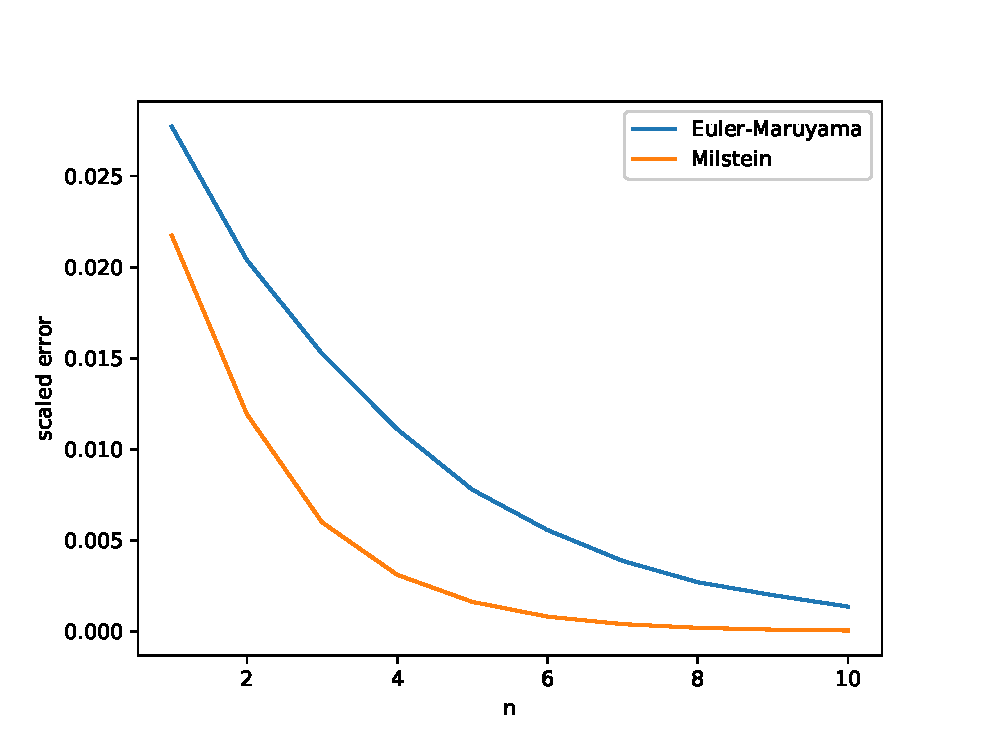
\includegraphics[width=\textwidth]{mc.eps}
  \caption{Scaled errors}
  \label{fig:1}
\end{figure}

\section{Multilevel Monte Carlo Simulation method}

To reduce estimation variance, multilevel monte carlo is promoted. In this section, multilevel monte carlo method is used to simulate the Black-Scholes model.

\subsection{Multilevel monte carlo}

As our aim is to estimate the expectation $\mathbb{E}[f(S_{n, T})]$, where $n$ means discretize the time with $M^{-n}$. In this report, $M=2$ is always supposed. In fact the expectation can be rewritten as:
\begin{align}
  \mathbb{E}[f(S_{n, T})]=\mathbb{E}[f(S_{1, T})] + \sum_{k=2}^{n}\mathbb{E}[f(S_{k, T})-f(S_{k-1, T})]
\end{align}

So the estimation of $f(S_{n, T})$ could be written as:
\begin{align}
  \widehat{f}(S_{n, T})=\frac{1}{N_{1}}\sum_{i=1}^{N_{1}}f(S_{1, T}^{(i)})+\sum_{k=2}^{n}\frac{1}{N_{k}}\sum_{i=1}^{N_{k}}[f(S_{k, T}^{(i)})-f(S_{k-1, T}^{(i)})]
\end{align}

To reduce variance, for each $k$, $f(S_{k,T}^{(i)})-f(S_{k-1,T}^{(i)})$ is independent with $f(S_{k-1,T}^{(j)})-f(S_{k-2,T}^{(j)})$, which means, the estimation of $f(S_{k,T}^{(i)})-f(S_{k-1,T}^{(i)})$ is depended on the path simulated by $f(S_{k, T}^{(i)})$ instead of $f(S_{k-1, T}^{(j)})$. So the variance of $\widehat{f}(S_{n, T})$ is:
\begin{align}
  Var[\widehat{f}(S_{n, T})]=\sum_{k=1}^{n}\frac{V_{k}}{N_{k}}
\end{align}
where $V_{k}=Var[f(S_{k, T})-f(S_{k-1, T})]$


\section{General formatting instructions}
\label{gen_inst}

The text must be confined within a rectangle 5.5~inches (33~picas) wide and
9~inches (54~picas) long. The left margin is 1.5~inch (9~picas).
Use 10~point type with a vertical spacing of 11~points. Times New Roman is the
preferred typeface throughout. Paragraphs are separated by 1/2~line space,
with no indentation.

Paper title is 17~point, in small caps and left-aligned.
All pages should start at 1~inch (6~picas) from the top of the page.

Authors' names are
set in boldface, and each name is placed above its corresponding
address. The lead author's name is to be listed first, and
the co-authors' names are set to follow. Authors sharing the
same address can be on the same line.

Please pay special attention to the instructions in section \ref{others}
regarding figures, tables, acknowledgments, and references.

\section{Headings: first level}
\label{headings}

First level headings are in small caps,
flush left and in point size 12. One line space before the first level
heading and 1/2~line space after the first level heading.

\subsection{Headings: second level}

Second level headings are in small caps,
flush left and in point size 10. One line space before the second level
heading and 1/2~line space after the second level heading.

\subsubsection{Headings: third level}

Third level headings are in small caps,
flush left and in point size 10. One line space before the third level
heading and 1/2~line space after the third level heading.

\section{Citations, figures, tables, references}
\label{others}

These instructions apply to everyone, regardless of the formatter being used.

\subsection{Citations within the text}

Citations within the text should be based on the \texttt{natbib} package
and include the authors' last names and year (with the ``et~al.'' construct
for more than two authors). When the authors or the publication are
included in the sentence, the citation should not be in parenthesis (as
in ``See \citet{Hinton06} for more information.''). Otherwise, the citation
should be in parenthesis (as in ``Deep learning shows promise to make progress towards AI~\citep{Bengio+chapter2007}.'').

The corresponding references are to be listed in alphabetical order of
authors, in the \textsc{References} section. As to the format of the
references themselves, any style is acceptable as long as it is used
consistently.

\subsection{Footnotes}

Indicate footnotes with a number\footnote{Sample of the first footnote} in the
text. Place the footnotes at the bottom of the page on which they appear.
Precede the footnote with a horizontal rule of 2~inches
(12~picas).\footnote{Sample of the second footnote}

\subsection{Figures}

All artwork must be neat, clean, and legible. Lines should be dark
enough for purposes of reproduction; art work should not be
hand-drawn. The figure number and caption always appear after the
figure. Place one line space before the figure caption, and one line
space after the figure. The figure caption is lower case (except for
first word and proper nouns); figures are numbered consecutively.

Make sure the figure caption does not get separated from the figure.
Leave sufficient space to avoid splitting the figure and figure caption.

You may use color figures.
However, it is best for the
figure captions and the paper body to make sense if the paper is printed
either in black/white or in color.
\begin{figure}[h]
\begin{center}
%\framebox[4.0in]{$\;$}
\fbox{\rule[-.5cm]{0cm}{4cm} \rule[-.5cm]{4cm}{0cm}}
\end{center}
\caption{Sample figure caption.}
\end{figure}

\subsection{Tables}

All tables must be centered, neat, clean and legible. Do not use hand-drawn
tables. The table number and title always appear before the table. See
Table~\ref{sample-table}.

Place one line space before the table title, one line space after the table
title, and one line space after the table. The table title must be lower case
(except for first word and proper nouns); tables are numbered consecutively.

\begin{table}[t]
\caption{Sample table title}
\label{sample-table}
\begin{center}
\begin{tabular}{ll}
\multicolumn{1}{c}{\bf PART}  &\multicolumn{1}{c}{\bf DESCRIPTION}
\\ \hline \\
Dendrite         &Input terminal \\
Axon             &Output terminal \\
Soma             &Cell body (contains cell nucleus) \\
\end{tabular}
\end{center}
\end{table}

\section{Final instructions}
Do not change any aspects of the formatting parameters in the style files.
In particular, do not modify the width or length of the rectangle the text
should fit into, and do not change font sizes (except perhaps in the
\textsc{References} section; see below). Please note that pages should be
numbered.

\section{Preparing PostScript or PDF files}

Please prepare PostScript or PDF files with paper size ``US Letter'', and
not, for example, ``A4''. The -t
letter option on dvips will produce US Letter files.

Consider directly generating PDF files using \verb+pdflatex+
(especially if you are a MiKTeX user).
PDF figures must be substituted for EPS figures, however.

Otherwise, please generate your PostScript and PDF files with the following commands:
\begin{verbatim}
dvips mypaper.dvi -t letter -Ppdf -G0 -o mypaper.ps
ps2pdf mypaper.ps mypaper.pdf
\end{verbatim}

\subsection{Margins in LaTeX}

Most of the margin problems come from figures positioned by hand using
\verb+\special+ or other commands. We suggest using the command
\verb+\includegraphics+
from the graphicx package. Always specify the figure width as a multiple of
the line width as in the example below using .eps graphics
\begin{verbatim}
   \usepackage[dvips]{graphicx} ...
   \includegraphics[width=0.8\linewidth]{myfile.eps}
\end{verbatim}
or % Apr 2009 addition
\begin{verbatim}
   \usepackage[pdftex]{graphicx} ...
   \includegraphics[width=0.8\linewidth]{myfile.pdf}
\end{verbatim}
for .pdf graphics.
See section~4.4 in the graphics bundle documentation (\url{http://www.ctan.org/tex-archive/macros/latex/required/graphics/grfguide.ps})

A number of width problems arise when LaTeX cannot properly hyphenate a
line. Please give LaTeX hyphenation hints using the \verb+\-+ command.


\subsubsection*{Acknowledgments}

Use unnumbered third level headings for the acknowledgments. All
acknowledgments, including those to funding agencies, go at the end of the paper.

\bibliography{iclr2018_conference}
\bibliographystyle{iclr2018_conference}

\end{document}
